\documentclass{article}
\usepackage[T1]{fontenc}
\usepackage[utf8]{inputenc}
\usepackage[english]{babel}
\usepackage{tikz}
\usepackage{times}
\usetikzlibrary{calc,through,backgrounds,positioning,fit}
\usetikzlibrary{shapes,arrows,shadows,calendar}

\begin{document}
\begin{tikzpicture}[scale=1.6,inner sep=1cm]
\centering
\coordinate (A) at (0,0);
\coordinate (B) at (1.5,0.5);
\coordinate (C) at (1.5,-0.5);

\draw (A) node [above right] {$\varphi$};
\draw (A) node [below right] {$\varphi$};
\draw (1,0) node[right] {1};
\draw  (A) -- (B) -- (C)  --cycle;

\end{tikzpicture} \qquad \qquad \qquad
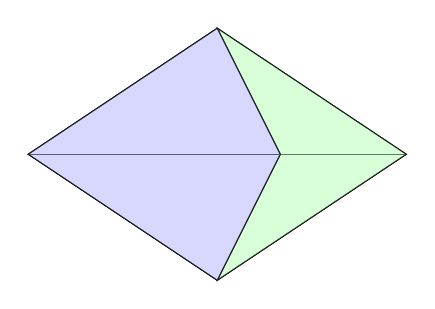
\begin{tikzpicture}[scale=1.6,inner sep=0.8cm]
\coordinate (A) at (0.5,0);
\coordinate (B) at (2,-1);
\coordinate (C) at (2,1);
\coordinate (D) at (3.5,0);
\coordinate (E) at (2.5,0);

\draw  (A) -- (B) -- (D) -- (C) --cycle;
\draw  (A) -- (D);
\draw  (B) -- (E) -- (C);

\filldraw [fill=green!30!white,opacity=0.5] (C) -- (D) -- (B) -- (E) -- cycle;
\filldraw [fill=blue!30!white,opacity=0.5] (C) -- (A) -- (B) -- (E) -- cycle;
\end{tikzpicture} \\\\
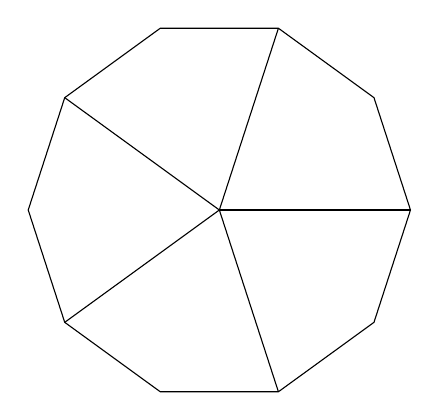
\begin{tikzpicture}[scale=1.5,inner sep=0.4mm]
\draw (0,0) -- (0:1.618) coordinate (p1);
\draw (0,0)  (36:1.618) coordinate (p2);
\draw (0,0) -- (72:1.618) coordinate (p3);
\draw (0,0)  (108:1.618) coordinate (p4);
\draw (0,0) -- (144:1.618) coordinate (p5);
\draw (0,0)  (180:1.618) coordinate (p6);
\draw (0,0) -- (216:1.618) coordinate (p7);
\draw (0,0)  (252:1.618) coordinate (p8);
\draw (0,0) -- (288:1.618) coordinate (p9);
\draw (0,0)  (324:1.618) coordinate (p10);
\draw (p1) -- (p2) -- (p3) -- (p4) -- (p5) -- (p6) -- (p7) -- (p8) -- (p9) -- (p10) -- (p1);
\end{tikzpicture} \qquad \qquad \qquad
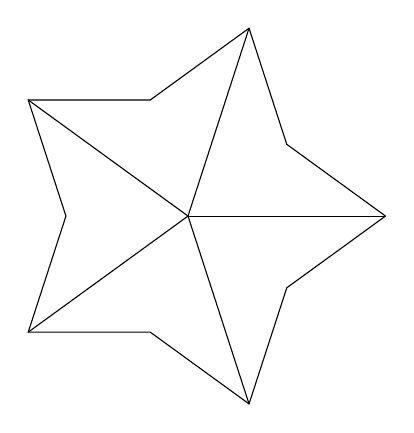
\begin{tikzpicture}[scale=1.55,inner sep=0.4mm]
\draw (0,0) -- (0:1.618) coordinate (p1);
\draw (0,0)  (36:1) coordinate (p2);
\draw (0,0) -- (72:1.618) coordinate (p3);
\draw (0,0)  (108:1) coordinate (p4);
\draw (0,0) -- (144:1.618) coordinate (p5);
\draw (0,0)  (180:1) coordinate (p6);
\draw (0,0) -- (216:1.618) coordinate (p7);
\draw (0,0)  (252:1) coordinate (p8);
\draw (0,0) -- (288:1.618) coordinate (p9);
\draw (0,0)  (324:1) coordinate (p10);
\draw (p1) -- (p2) -- (p3) -- (p4) -- (p5) -- (p6) -- (p7) -- (p8) -- (p9) -- (p10) -- (p1);
\end{tikzpicture}  


\end{document}